
%!TEX encoding = UTF-8 Unicode
%!TEX root = ../exercises.tex

\ifPreSolution

\Exercise{\ExeWeekFIVE}\label{exe:W05}

\begin{Goals}
%!TEX encoding = UTF-8 Unicode

%!TEX root = ../compendium1.tex

\item Kunna deklarera klasser med klassparametrar.
\item Kunna skapa instanser med \code{new}.
\item Kunna ge argument vid instansiering.
\item Förstå innebörden av referensvariabler och värdet \code{null}.

\item Kunna använda nyckelordet \code{private} för att styra synlighet av attribut och konstruktorparametrar.

\item Förstå syftet med getters och setters.
\item Kunna förklara accessregler för kompanjonsobjekt.
\item Kunna skapa fabriksmetod i kompanjonsobjekt.
\item Känna till nyttan med en privat konstruktor.

%\item Kunna implementera en klass utifrån en specifikation.
\item Förstå skillnaden mellan referenslikhet och strukturlikhet.
\item Känna till skillnaden mellan \code{==} och \code{eq}, samt \code{!=} och \code{ne}.

\item Kunna förklara hur case-klasser hanterar instansiering.
\item Känna till hur case-klasser hanterar likhet.

\end{Goals}

\begin{Preparations}
\item \StudyTheory{05}
\end{Preparations}

\else


\ExerciseSolution{\ExeWeekFIVE}


\fi


\BasicTasks %%%%%%%%%%%


\WHAT{Para ihop begrepp med beskrivning.}

\QUESTBEGIN

\Task \what

\vspace{1em}\noindent Koppla varje begrepp med den (förenklade) beskrivning som passar bäst:

\begin{ConceptConnections}
  klass & 1 & & A & hjälpfunktion för att anropa konstruktor \\ 
  instans & 2 & & B & upplaga av ett objekt med eget tillståndsminne \\ 
  konstruktor & 3 & & C & skapar instans, allokerar plats för tillståndsminne \\ 
  klassparameter & 4 & & D & olika instanser anses lika om de har samma tillstånd \\ 
  fabriksmetod & 5 & & E & en mall för att skapa flera instanser av samma typ \\ 
  referenslikhet & 6 & & F & ge argument vid konstruktion, initialisera tillstånd \\ 
  innehållslikhet & 7 & & G & ser privata medlemmar i klassen med samma namn \\ 
  case-klass & 8 & & H & slipper skriva new; automatisk innehållslikhet \\ 
  kompanjonsobjekt & 9 & & I & instanser anses olika även om de har samma tillstånd \\ 
\end{ConceptConnections}

\SOLUTION

\TaskSolved \what

\begin{ConceptConnections}
  klass & 1 & ~~\Large$\leadsto$~~ &  K & en mall för att skapa flera instanser av samma typ \\ 
  instans & 2 & ~~\Large$\leadsto$~~ &  H & upplaga av ett objekt med eget tillståndsminne \\ 
  konstruktor & 3 & ~~\Large$\leadsto$~~ &  L & skapar instans, allokerar plats för tillståndsminne \\ 
  klassparameter & 4 & ~~\Large$\leadsto$~~ &  E & binds till argument som ges vid konstruktion \\ 
  referenslikhet & 5 & ~~\Large$\leadsto$~~ &  J & instanser anses olika även om tillstånden är lika \\ 
  innehållslikhet & 6 & ~~\Large$\leadsto$~~ &  A & instanser anses lika om de har samma tillstånd \\ 
  case-klass & 7 & ~~\Large$\leadsto$~~ &  F & slipper skriva new; automatisk innehållslikhet \\ 
  getter & 8 & ~~\Large$\leadsto$~~ &  I & indirekt åtkomst av attributvärde \\ 
  setter & 9 & ~~\Large$\leadsto$~~ &  C & indirekt tilldelning av attributvärde \\ 
  kompanjonsobjekt & 10 & ~~\Large$\leadsto$~~ &  B & ser privata medlemmar i klass med samma namn \\ 
  fabriksmetod & 11 & ~~\Large$\leadsto$~~ &  M & hjälpfunktion för indirekt konstruktonsanrop \\ 
  \code|null| & 12 & ~~\Large$\leadsto$~~ &  G & ett värde som ej refererar till någon instans \\ 
  \code|new| & 13 & ~~\Large$\leadsto$~~ &  D & nyckelord vid direkt instansiering av klass \\ 
\end{ConceptConnections}

\QUESTEND


\WHAT{Klass och instans.}

\QUESTBEGIN

\Task \what~Du har i övning \texttt{\ExeWeekFOUR}~sett hur singelobjekt i en egen namnrymd  kan samla funktioner (metoder) och ha tillstånd (attribut). Men singelobjekt finns bara i en upplaga.

Vill du kunna skapa många objekt av samma typ behöver du en \emph{klass}. En objektupplaga som skapats ur en klass kallas en \emph{instans} av klassen. Varje instans har sitt eget tillstånd.

Deklarera singelobjektet och klassen nedan i REPL.

\begin{Code}
object Singelpunkt { var x = 1; var y = 2 }
class  Punkt       { var x = 3; var y = 2 }
\end{Code}

\Subtask  Antag att uttrycken till vänster evalueras uppifrån och ned. Vilket resultat till höger hör ihop med respektive uttryck? Prova i REPL om du är osäker.\footnote{Strängen efter \code{@}-tecknet är en hexadecimal representation av det heltal som tillordnas varje objekt för att systemet ska kunna särskilja olika instanser. \url{https://stackoverflow.com/questions/4712139}}


\begin{ConceptConnections}
  \code|Singelpunkt.x               | & 1 & & A & \code|2| \\ 
  \code|Punkt.x                     | & 2 & & B & \verb|error: not found: type| \\ 
  \code|val p  = new Singelpunkt    | & 3 & & C & \code|1| \\ 
  \code|val p1 = new Punkt          | & 4 & & D & \verb|p2: Punkt = Punkt@51ab04bd| \\ 
  \code|val p2 = new Punkt          | & 5 & & E & \code|java.lang.NullPointerException| \\ 
  \code|{ p1.x = 1; p2.x }          | & 6 & & F & \verb|p1: Punkt = Punkt@27a1a53c| \\ 
  \code|(new Punkt).y               | & 7 & & G & \code|3| \\ 
  \code|{ val p: Punkt = null; p.x }| & 8 & & H & \code|error: not found: value| \\ 
\end{ConceptConnections}

\Subtask Vid tre tillfällen blir det fel. Varför? Är det kompileringsfel eller exekveringsfel?

\SOLUTION

\TaskSolved \what

\SubtaskSolved

\begin{ConceptConnections}
  \code|Singelpunkt.x               | & 1 & ~~\Large$\leadsto$~~ &  H & \code|1| \\ 
  \code|Punkt.x                     | & 2 & ~~\Large$\leadsto$~~ &  B & \code|error: not found: value| \\ 
  \code|val p  = new Singelpunkt    | & 3 & ~~\Large$\leadsto$~~ &  A & \verb|error: not found: type| \\ 
  \code|val p1 = new Punkt          | & 4 & ~~\Large$\leadsto$~~ &  F & \verb|p1: Punkt = Punkt@27a1a53c| \\ 
  \code|val p2 = new Punkt          | & 5 & ~~\Large$\leadsto$~~ &  D & \verb|p2: Punkt = Punkt@51ab04bd| \\ 
  \code|{ p1.x = 1; p2.x }          | & 6 & ~~\Large$\leadsto$~~ &  E & \code|3| \\ 
  \code|(new Punkt).y               | & 7 & ~~\Large$\leadsto$~~ &  G & \code|2| \\ 
  \code|{ val p: Punkt = null; p.x }| & 8 & ~~\Large$\leadsto$~~ &  C & \code|java.lang.NullPointerException| \\ 
\end{ConceptConnections}

\SubtaskSolved

\noindent\begin{tabular}{l l p{5cm}}

~\\ \emph{fel} & \emph{typ} & \emph{förklaring} \\\hline

\code|error: not found: value|
& kompileringsfel & det finns ingen instans med namnet \code|Punkt|\\

\verb|error: not found: type|
& kompileringsfel & det finns ingen klass som heter \code|Singelpunkt|\\

\code|NullPointerException|
& körtidsfel & det går inte att referera attribut i en instans som inte finns\\

\end{tabular}

\QUESTEND



\WHAT{Klassparametrar.}

\QUESTBEGIN

\Task \what~Klassen punkt i föregående uppgift är inte så smidig att använda eftersom man först \emph{efter} instansiering kan ge attributen \code{x} och \code{y} de koordinatvärden man önskar och detta måste ske med explicita tilldelningssatser.

Detta problem kan du lösa med \emph{klassparametrar} som låter dig initialisera attributen med konstruktionsargument och på så sätt ange ett initialtillstånd direkt i samband med instansiering.

Deklarera klassen nedan i REPL.

\begin{Code}
class Point(var x: Int, var y: Int)
\end{Code}


\Subtask  Antag att uttrycken till vänster evalueras uppifrån och ned. Vilket resultat till höger hör ihop med respektive uttryck? Prova i REPL om du är osäker.

\begin{ConceptConnections}
  \code|val p1 = Point(1, 2)        | & 1 & & A & \verb|p2: Point = Point@218cf600| \\ 
  \code|val p2 = new Point          | & 2 & & B & \code|error: not enough arguments| \\ 
  \code|val p1 = new Point(1, 2)    | & 3 & & C & \code|2| \\ 
  \code|val p2 = new Point(3, 4)    | & 4 & & D & \code|error: not found: value| \\ 
  \code|p2.x - p1.x                 | & 5 & & E & \code|1| \\ 
  \code|(new Point(0, 1)).y         | & 6 & & F & \code|error: too many arguments| \\ 
  \code|new Point(0, 1, 2)          | & 7 & & G & \verb|p1: Point = Point@30ef773e| \\ 
\end{ConceptConnections}

\Subtask Vid tre tillfällen blir det fel. Varför? Är det kompileringsfel eller exekveringsfel?

\SOLUTION

\TaskSolved \what

\SubtaskSolved

\begin{ConceptConnections}
  \code|val p1 = Point(1, 2)        | & 1 & ~~\Large$\leadsto$~~ &  B & \code|error: not found: value| \\ 
  \code|val p2 = new Point          | & 2 & ~~\Large$\leadsto$~~ &  E & \code|error: not enough arguments| \\ 
  \code|val p1 = new Point(1, 2)    | & 3 & ~~\Large$\leadsto$~~ &  F & \verb|p1: Point = Point@30ef773e| \\ 
  \code|val p2 = new Point(3, 4)    | & 4 & ~~\Large$\leadsto$~~ &  C & \verb|p2: Point = Point@218cf600| \\ 
  \code|p2.x - p1.x                 | & 5 & ~~\Large$\leadsto$~~ &  D & \code|2| \\ 
  \code|(new Point(0, 1)).y         | & 6 & ~~\Large$\leadsto$~~ &  G & \code|1| \\ 
  \code|new Point(0, 1, 2)          | & 7 & ~~\Large$\leadsto$~~ &  A & \code|error: too many arguments| \\ 
\end{ConceptConnections}

\SubtaskSolved

\noindent\begin{tabular}{l l p{5cm}}

  ~\\ \emph{fel} & \emph{typ} & \emph{förklaring} \\\hline

  \code|error: not found: value|
  & kompileringsfel & det finns ingen instans med namnet \code|Point|\\

  \verb|error: not enough arguments|
  & kompileringsfel  & du måste ge argument vid konstruktion av klassen \code|Point| \\

  \code|error: too many arguments|
  & kompileringsfel & antalet argument stämmer ej överens med antalet klassparametrar\\

\end{tabular}

\QUESTEND



\WHAT{Oföränderlig klass med defaultargument.}

\QUESTBEGIN

\Task \what~Det du tidigare lärt dig om parametrar och argument är tillämpligt även på klassparametrar, t.ex. defaultargument och namngivna argument. Man kan dessutom framför klassparametrar använda synlighetsmodifieraren \code{private} och nyckelorden \code{var} och \code{val}.

Om inget anges framför en klassparameter är det \code{private val} som gäller\footnote{För case-klasser, som vi ska se snart, är det i stället \code{val} som gäller (alltså inte \code{private}).}.

Deklarera nedan klass i REPL.

\begin{Code}
class Point3D(val x: Int = 0, val y: Int = 0, z: Int = 0)
\end{Code}

\Subtask Antag att uttrycken till vänster evalueras uppifrån och ned. Vilket resultat till höger hör ihop med respektive uttryck? Prova i REPL om du är osäker.

\begin{ConceptConnections}
  \code|val p1 = new Point3D        | & 1 & & A & \code|false| \\ 
  \code|val p2 = new Point3D(y = 1) | & 2 & & B & \code|Reassignment to val| \\
  \code|(new Point3D(z = 2)).z      | & 3 & & C & \verb|p1: Point3D = Point3D@2eb37eee| \\ 
  \code|p2.y = 0                    | & 4 & & D & \code|true| \\ 
  \code|p2.y == 0                   | & 5 & & E & \code|value cannot be accessed| \\
  \code|p1.x == (new Point3D).x     | & 6 & & F & \verb|p2: Point3D = Point3D@65a9e8d7|

\end{ConceptConnections}

\Subtask Vad är problemet med ovan klass om man vill använda den för att representera punkter i 3 dimensioner?

\SOLUTION

\TaskSolved \what~

\SubtaskSolved

\begin{ConceptConnections}
  \code|val p1 = new Point3D        | & 1 & ~~\Large$\leadsto$~~ &  E & \verb|p1: Point3D = Point3D@2eb37eee| \\ 
  \code|val p2 = new Point3D(y = 1) | & 2 & ~~\Large$\leadsto$~~ &  A & \verb|p2: Point3D = Point3D@65a9e8d7| \\ 
  \code|(new Point3D(z = 2)).z      | & 3 & ~~\Large$\leadsto$~~ &  B & \code|error: not found: value| \\ 
  \code|p2.y = 0                    | & 4 & ~~\Large$\leadsto$~~ &  C & \code|error: reassignment to val| \\ 
  \code|p2.y == 0                   | & 5 & ~~\Large$\leadsto$~~ &  F & \code|false| \\ 
  \code|p1.x == (new Point3D).x     | & 6 & ~~\Large$\leadsto$~~ &  D & \code|true| \\ 
\end{ConceptConnections}

\SubtaskSolved Problemet är att så som klassen \code{Point3D} är deklarerad går det inte att avläsa \code{z}-koordinaten efter att en instans konstruerats. Det vore bättre om även \code{z}-attributet är \code{val}.

\QUESTEND



\WHAT{Case-klass, \code{this}, likhet, \code{toString} och kompanjonsobjekt.}

\QUESTBEGIN

\Task \what~\\Klistra in nedan klasser i REPL.

\begin{Code}
case class Pt(x: Int = 0, y: Int = 0) {
  def moved(dx: Int = 0, dy: Int = 0): Pt = Pt(x + dx, y + dy)
}

class MutablePt(private var p: (Int, Int) = (0, 0)) {
  def x: Int = p._1
  def y: Int = p._2
  def move(dx: Int = 0, dy: Int = 0) = { p = (x + dx, y+ dy); this }
  override def toString = s"MPt($x,$y)"
}
\end{Code}

\Subtask
Antag att uttrycken till vänster evalueras uppifrån och ned. Vilket REPL-svar till höger hör ihop med respektive uttryck? Prova i REPL om du är osäker.

\begin{ConceptConnections}
  \code|val p1 = Pt(1, 2)             | & 1 & & A & \code|MPt(5,6)| \\ 
  \code|val p2 = Pt(y = 3)            | & 2 & & B & \code|false| \\ 
  \code|val p3 = MutablePt(5, 6)      | & 3 & & C & \code|Pt(0,3)| \\ 
  \code|val p4 = Mutable()            | & 4 & & D & \code|Not found| \\ 
  \code|p2.moved(dx = 1) == Pt(1, 3)  | & 5 & & E & \code|Pt(1,2)| \\ 
  \code|p3.move(dy = 1) == MutablePt(5, 7)| & 6 & & F & \code|true| \\ 
\end{ConceptConnections}

\Subtask Vilken returtyp kommer kompilatorn härleda för funktionen MutablePt.move?

\Subtask Implementera en fabriksmetod \code{apply} i ett kompanjonsobjekt till klassen \code{MutablePt} som gör att du inte behöver skriva \code{new} när du skapar instanser.

\SOLUTION

\TaskSolved \what~\TODO

\SubtaskSolved \TODO

\begin{ConceptConnections}
  \code|val p1 = new Pt(1,2)        | & 1 & ~~\Large$\leadsto$~~ &  A & \code|Pt(1,2)| \\ 
  \code|val p2 = Pt(y=3)            | & 2 & ~~\Large$\leadsto$~~ &  B & \code|Pt(0,3)| \\ 
  \code|val p3 = new MutablePt(5, 6)| & 3 & ~~\Large$\leadsto$~~ &  D & \code|MPt(5,6)| \\ 
  \code|val p4 = Mutable()          | & 4 & ~~\Large$\leadsto$~~ &  E & \code|error: not found: value| \\ 
  \code|p2.moved(dx=1) == Pt(1, 3)  | & 5 & ~~\Large$\leadsto$~~ &  G & \code|true| \\ 
  \code|p3.move(dy=1) == new MutablePt(5,7)| & 6 & ~~\Large$\leadsto$~~ &  F & \code|false| \\ 
  \code|p2 == p3                      | & 7 & ~~\Large$\leadsto$~~ &  C & \verb|warning: always false| \\ 
\end{ConceptConnections}


\SubtaskSolved \TODO

\SubtaskSolved \TODO

\QUESTEND


\WHAT{Skapa en punktklass att använda på veckans laboration.}

\QUESTBEGIN

\Task \what~
Du ska som förberedelse till laborationen skapa den oföränderliga case-klassen \code{Point} som ska beskriva en koordinat i ett kartesiskt koordinatsystem\footnote{\url{https://sv.wikipedia.org/wiki/Kartesiskt_koordinatsystem}}. Skapa kod med hjälp av en editor, t.ex. \code{atom}, i filen  \code{Point.scala} enligt följande riktlinjer:
\begin{enumerate}[noitemsep]
\item \code{Point} ska ligga i paketet \code{graphics}.

\item \code{Point} ska ha följande två publika, oföränderliga klassparametrar:
\begin{itemize}[nolistsep, noitemsep]
\item \code{x: Double} för x-koordinaten.
\item \code{y: Double} för y-koordinaten.
\end{itemize}

\item \code{Point} ska ha följande publika medlemmar (två oföränderliga attribut och två metoder):
\begin{itemize}[nolistsep, noitemsep]
\item \code{val r: Double} ska ge motsvarande polära kordinatens%
\footnote{\url{https://sv.wikipedia.org/wiki/Pol\%C3\%A4ra\_koordinater}}
 avstånd till origo.
\item \code{val theta: Double} ska ge polära kordinatens vinkel i radianer.
\item \code{def negY: Point} ska ge en ny punkt med y-koordinaten negerad.
\item \code{def +(p: Point): Point} ska ge en ny punkt vars koordinat är summan av x- respektive y-kordinaterna för denna instans och punkten \code{p}.
\end{itemize}

\item \code{Point} ska ha ett kompanjonsobjekt med en metod som konstruerar en punkt från polära koortdinater. Metoden ska ha detta huvud: \\\code{def polar(r: Double, theta: Double): Point}

\end{enumerate}

\noindent Tips vid implementation och senare användning:
\begin{itemize}
\item Du har nytta av metoderna \code{math.hypot(x, y)} och \code{math.atan2(y, x)} vid omvandling till polära koordinater.

\item Du har nytta av metoderna \code{math.cos(x)} och \code{math.sin(y)} vid omvandling från polära koordinater.

\item Attributet \code{negY} kommer att underlätta för dig när du i metoden \code{draw} i klassen \code{Turtle} ska omvandla en punkt till fönsterkoordinater där y-axeln är omvänd jämfört med kartesiska koordinater.

\item Notera att klassens attribut är av typen \code{Double} och inte \code{Int}, trots att vi senare ska använda punkten för att beskriva en diskret pixelposition. Anledningen till detta är att det kan uppstå avrundningsfel vid numeriska beräkningar. Detta blir särskilt märkbart vid upprepad räkning med små värden, t.ex. när man ritar en approximerad cirkel med många linjesegment.
\end{itemize}

\SOLUTION

\TaskSolved \what~\TODO

\QUESTEND



\AdvancedTasks %%%%%%%%%%%%%%%%%%%%%%%%%%%%%%%%%%%%%%%%%%%%%%%%%%%%%%%%%%%%%%%%%

\WHAT{Ändra attributrepresentation. Privat konstruktor}

\QUESTBEGIN

\Task \what~Kim Kodkunnig skapade för länge sedan denna punktklass som används på många ställen i befintlig kod:

\begin{Code}
class Point private (val x: Int, val y: Int)
object Point {
  def apply(x: Int = 0, y: Int = 0): Point = new Point(x, y)
  def origo = apply()
}
\end{Code}

\Subtask Vad händer om du försöker instansiera Kim Kodkunnigs klass i din egen kod direkt med nyckelordet \code{new}?

\Subtask Varför använder Kim Kodkunnig ett kompanjonsobjekt med en fabriksmetod? Vilka accessregler gäller mellan ett kompanjonsobjekt och klassen med samma namn?

\Subtask Hjälp Kim Kodkunnig att ändra attributrepresentationen så att det oföränderliga tillståndet utgörs av en 2-tupel \code{val p: (Int, Int)} i stället. Befintlig kod ska inte behöva ändras och klassen \code{Point} ska bete sig från ''utsidan'' precis som innan.

\SOLUTION

\TaskSolved \what~

\SubtaskSolved Det blir kompileringsfel eftersom konstruktorn är privat.
\begin{REPL}
scala> :paste

class Point private (val x: Int, val y: Int)
object Point {
  def apply(x: Int = 0, y: Int = 0): Point = new Point(x, y)
  def origo = apply()
}

scala> new Point(0,0)
<console>:14: error: constructor Point in class Point cannot be accessed
\end{REPL}

\SubtaskSolved
\begin{itemize}
  \item Genom att ha en privat konstruktor och bara göra indirekt instansiering via fakriksmetod är det möjligt att ändra attributrepresentation i framtiden utan att befintlig kod behöver ändras.

  \item Med en \code{apply}-metod i kompansjonsobjektet kan man instansiera genom att skriva \code{Point(1, 2)} utan new.

  \item Accessreglerna för kompanjonsobjekt är sådana att kompanjoner ser varandras privata delar.
\end{itemize}

\SubtaskSolved

\begin{Code}
class Point private (private val p: (Int, Int)) {
  def x: Int = p._1
  def y: Int = p._2
}
object Point {
  def apply(x: Int = 0, y: Int = 0): Point = new Point(x, y)
  def origo = apply()
}
\end{Code}

\QUESTEND


\subsection{\TODO värdera nedan uppgifter}


\WHAT{Instansiering med \code{new} och värdet \code{null}.}

\QUESTBEGIN

\Task  \what~  Man skapar instanser av klasser med \code{new}. Då anropas konstruktorn och plats reserveras i datorns minne för objektet. Variabler av referenstyp som inte refererar till något objekt har värdet \code{null}.

\Subtask Vad händer nedan? Vilka rader ger felmeddelande och i så fall hur lyder felmeddelandet?

\begin{REPL}
scala> class Gurka(val vikt: Int)
scala> var g: Gurka = null
scala> g.vikt
scala> g = new Gurka(42)
scala> g.vikt
scala> g = null
scala> g.vikt
\end{REPL}

\Subtask\Pen Rita minnessituationen efter raderna 2, 4, 6.

\SOLUTION


\TaskSolved \what


\SubtaskSolved  Rad 3 och 7 ger båda felmeddelandet "java.lang.NullPointerException". Detta eftersom \code{g} i båda fallen inte innehåller en referens till en \code{Gurka} utan pekar på inget -- "null".

\SubtaskSolved  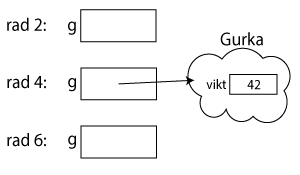
\includegraphics[scale=0.6]{../img/w06-solutions/1b}


\QUESTEND




%%<AUTOEXTRACTED by mergesolu>%%      % uppgift 1




\WHAT{Klasser och instanser.}

\QUESTBEGIN

\Task  \what~

\Subtask Vad händer nedan?
\begin{REPL}
scala> :pa
class Arm(val ärTillVänster: Boolean)
class Ben(val ärTillVänster: Boolean)
class Huvud(val harHår: Boolean)
class Rymdvarelse {
  var arm1 = new Arm(true)
  var arm2 = new Arm(false)
  var ben1 = new Ben(true)
  var ben2 = new Ben(false)
  var huvud1 = new Huvud(false)
  var huvud2 = new Huvud(true)
  def ärSkallig = !huvud1.harHår && !huvud2.harHår
}
scala> val alien = new Rymdvarelse
scala> alien.ärSkallig
scala> val predator = new Rymdvarelse
scala> predator.ärSkallig
scala> predator.huvud2 = alien.huvud1
scala> predator.ärSkallig
\end{REPL}

\Subtask\Pen Rita minnessituationen efter rad 18.

\Subtask\Pen Vad händer så småningom med det ursprungliga huvud2-objektet i predator efter tilldelningen på rad 18? Går det att referera till detta objekt på något sätt?


\SOLUTION


\TaskSolved \what


\SubtaskSolved  Vi skapar två rymdvarelser, \code{alien} och \code{predator}, med två ben, två armar samt två huvuden (där det ena är skalligt och det andra har hår) vardera. Efter det är varken \code{alien} eller \code{predator} skallig eftersom båda har ett huvud med hår. Sen låter man referensen till \code{predator}s huvud med hår referera till aliens huvud utan hår. Nu är predator helt skallig.

\SubtaskSolved   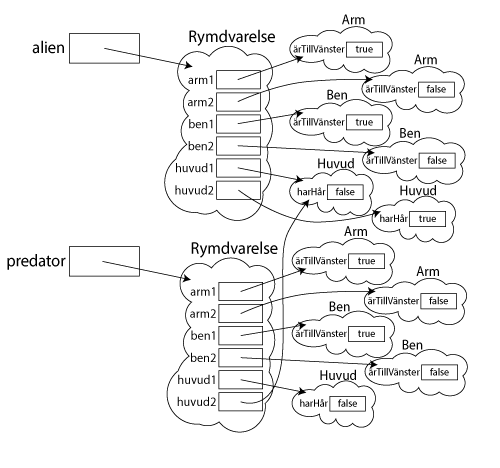
\includegraphics[scale=0.7]{../img/w06-solutions/2b}

\SubtaskSolved  Eftersom det inte längre finns någon referens som pekar på det objektet kommer Garbage Collector ta hand om det och kommer förr eller senare skrivas över av något annat som behöver sparas. Nej, det går inte att komma åt.

% uppgift 3

\QUESTEND




%%<AUTOEXTRACTED by mergesolu>%%      % uppgift 2




\WHAT{Synlighet i primärkonstruktorer.}

\QUESTBEGIN

\Task  \what~  Undersök nedan vad nyckelorden \code{val} och \code{private} får för konsekvenser. Förklara vad som händer. Vilka rader ger vilka felmeddelanden?

\begin{REPL}
scala> class Gurka1(vikt: Int)
scala> new Gurka1(42).vikt
scala> class Gurka2(val vikt: Int)
scala> new Gurka2(42).vikt
scala> class Gurka3(private val vikt: Int)
scala> new Gurka3(42).vikt
scala> class Gurka4(private val vikt: Int, kompis: Gurka4){
         def kompisVikt = kompis.vikt
       }
scala> val ingenGurka: Gurka4 = null
scala> new Gurka4(42, ingenGurka).kompisVikt
scala> new Gurka4(42, new Gurka4(84, null)).kompisVikt
scala> class Gurka5(private[this] val vikt: Int, kompis: Gurka5){
         def kompisVikt = kompis.vikt
       }
scala> class Gurka6 private (vikt: Int)
scala> new Gurka6(42)
scala> :pa
class Gurka7 private (var vikt: Int)
object Gurka7 {
  def apply(vikt: Int) = {
    require(vikt >= 0, s"negativ vikt: $vikt")
    new Gurka7(vikt)
  }
}
scala> new Gurka7(-42)
scala> Gurka7(-42)
scala> val g = Gurka7(42)
scala> g.vikt
scala> g.vikt = -1
scala> g.vikt
\end{REPL}


\SOLUTION


\TaskSolved \what
 Rad 2:
\begin{REPL}
	error: value vikt is not a member of Gurka1
\end{REPL}
Detta eftersom om man varken väljer att skriva \code{val} eller \code{var} skapar inte scala någon getter eller setter (metoder för att läsa/ändra en variabel) och därför ser det ut som att vikt inte finns för kompilatorn.

Rad 4: Denna rad skapar inte en error eftersom om man skriver \code{val} innan variabeln skapas en getter automatiskt och man kan därför komma åt \code{vikt}.

Rad 6:
\begin{REPL}
	error: value vikt in class Gurka3 cannot be accessed in Gurka3
\end{REPL}
I detta fallet skapas en \code{getter} men eftersom accessnivån sätts till \code{private} vet kompilatorn att man inte får komma åt variabeln utifrån.

Rad 11:
\begin{REPL}
	java.lang.NullPointerException
\end{REPL}
Detta eftersom \code{kompis} är \code{ingenGurka} som inte pekar på något objekt och när man då försöker komma åt ett attribut från den kommer det inte funka.

Rad 12: Kommer inte generera en error eftersom när man kallar \code{kompisVikt} (som är \code{public}) försöker den komma åt \code{Gurka4(84, null).vikt}. \code{vikt} är \code{private val} vilket innebär att det har en getter och eftersom huvudobjektet också är av typen \code{Gurka4} är accessnivån tillräckligt hög.

Rad 13:
\begin{REPL}
	error: value vikt is not a member of Gurka5
\end{REPL}
När man sätter ett attribut till \code{private[this]} tillåts inte ens objekt av samma typ att komma åt variabeln och därför får man en error som säger att den inte finns.

Rad 17:
\begin{REPL}
	error: constructor Gurka6 in class Gurka6 cannot be accessed in object
\end{REPL}
Eftersom man satt klassparametrarna till \code{private} kan man inte komma åt konstruktorn och därför får man en error.

Rad 26:
\begin{REPL}
	error: constructor Gurka7 in class Gurka7 cannot be accessed in object
\end{REPL}
Samma anledning som på rad 17.

Rad 27:
\begin{REPL}
	java.lang.IllegalArgumentException: requirement failed: negativ vikt: -42
\end{REPL}
Kompanjonsobjektet har en requirement på att \code{vikt >= 0} vilket innebär att om det inte stämmer kommer man få en error av typen \code{IllegalArgumentException}.

Rad 30: Anledningen till att man kan sätta vikten till något negativt är att checken om det är negativt endast görs när man skapar \code{Gurka7} vilket innebär att i efterhand kan man ändra den till vilket värde som helst (av typen \code{Int}).


\QUESTEND






\WHAT{Egendefinierad setter kombinerat med privat konstruktor.}

\QUESTBEGIN

\Task  \what~

\Subtask Förklara vad som händer nedan. Vilka rader ger vilka felmeddelanden?
\begin{REPL}
scala> :pa
class Gurka8 private (private var _vikt: Int) {
  def vikt = _vikt
  def vikt_=(v: Int): Unit = {
    require(v >= 0, s"negativ vikt: $v")
    _vikt = v
  }
}

object Gurka8 {
  def apply(vikt: Int) = {
    require(vikt >= 0, s"negativ vikt: $vikt")
    new Gurka8(vikt)
  }
}
scala> val g = Gurka8(-42)
scala> val g = Gurka8(42)
scala> g.vikt
scala> g.vikt = 0
scala> g.vikt = -1
scala> g.vikt += 42
scala> g.vikt -= 1000
\end{REPL}

\Subtask\Pen Vad är fördelen med möjligheten att skapa egendefinierade setters?

\SOLUTION


\TaskSolved \what


\SubtaskSolved  Rad 16:
\begin{REPL}
	java.lang.IllegalArgumentException: requirement failed: negativ vikt: -42
\end{REPL}
Kompanjonsobjektet har en requirement på att \code{vikt >= 0} vilket innebär att om det inte stämmer kommer man få en error.

Rad 20:
\begin{REPL}
	java.lang.IllegalArgumentException: requirement failed: negativ vikt: -1
\end{REPL}
Eftersom settern har implementerat ett krav på att vikten måste vara större eller lika med 0 får man en error när man försöker sätta den till -1.

Rad 22:
\begin{REPL}
	java.lang.IllegalArgumentException: requirement failed: negativ vikt: -958
\end{REPL}
Eftersom 42-1000 är mindre än noll får man en error.

\SubtaskSolved  Man kan sätta egna mer specifika krav på vad som får göras med värdena så man har större koll på att inget oväntat händer.

% uppgift 5

\QUESTEND




%%<AUTOEXTRACTED by mergesolu>%%      % uppgift 4




\WHAT{En oföränderlig kvadrat med alternativ fabriksmetod.}

\QUESTBEGIN

\Task \label{task:Square} \what~

\Subtask Implementera klassen \code{Square} enligt nedan specifikation. Gör  implementationen i en kodeditor, så som \code{gedit}, och klistra in klassen i Scala REPL efter kommandot \code{:pa} (förkortning av \code{:paste}). På så sätt blir \code{object Square} ett kompanjonsobjekt till \code{class Square}.

\begin{ScalaSpec}{Square}
/** A class representing a square object with position and side. */
class Square(val x: Int, val y: Int, val side: Int) {
  /** The area of this Square */
  val area: Int = ???

  /** Creates a new Square moved to position (x + dx, y + dy) */
  def move(dx: Int, dy: Int): Square = ???

  /** Tests if this Square has equal size as that Square */
  def isEqualSizeAs(that: Square): Boolean = ???

  /** Multiplies the side with factor and rounded to nearest integer */
  def scale(factor: Double): Square = ???

  /** A string representation of this Square */
  override def toString: String = ???
}

object Square {
  /** A square placed in origin with size 1 */
  val unit: Square = ???

  /** Constructs a new Square object at (x, y) with size side */
  def apply(x: Int, y: Int, side: Int): Square = ???

  /** Constructs a new Square object at (0, 0) with side 1 */
  def apply(): Square = ???
}
\end{ScalaSpec}

\Subtask Testa din kvadrat enligt nedan. Förklara vad som händer.

\begin{REPL}
scala> val (s1, s2) = (Square(), Square(1, 10, 1))
scala> val s3 = s1.move(1,-5)
scala> s1 isEqualSizeAs s3
scala> s2 isEqualSizeAs s1
scala> s1 isEqualSizeAs Square.unit
scala> s2.scale(math.Pi) isEqualSizeAs s2
scala> s2.scale(math.Pi) isEqualSizeAs s2.scale(math.Pi)
\end{REPL}

\SOLUTION


\TaskSolved \what
 \begin{CodeSmall}
	class Square(val x: Int, val y: Int, val side: Int) {
		val area: Int = side*side

		def move(dx: Int, dy: Int): Square = new Square(x + dx, y + dy, side)

		def isEqualSizeAs(that: Square): Boolean = this.side == that.side

		def scale(factor: Double): Square = new Square(x, y, (side*factor).toInt)

		override def toString: String = s"Square(x: $x, y: $y, side: $side)"
	}

	object Square {
		val unit: Square = new Square(0, 0, 1)

		def apply(x: Int, y: Int, side: Int): Square = new Square(x, y, side)

		def apply(): Square = new Square(0, 0, 1)
	}
\end{CodeSmall}

Eftersom \code{s1}, \code{s2}, \code{s3} och \code{Square.unit} alla har en sida med längden 1 så kommer rad 3-5 returnera \code{true}. Rad 6 kommer returnera \code{false} eftersom \code{s2.scale(math.Pi)} sida är $\pi$ och \code{s2} fortfarande har sidan 1. Rad 7 kommer däremot returnera \code{true} då båda har sidan $\pi$.


\QUESTEND






\WHAT{Referenslikhet versus strukturlikhet.}

\QUESTBEGIN

\Task  \what~  Metoden \code{==} på case-klasser ger \textbf{strukturlikhet} (även kallad innehållslikhet) så att \emph{innehållet} i klassens klassparametrar jämförs om de har lika värde, medan för vanliga klasser ger metoden \code{==} \textbf{referenslikhet} där olika objekt är olika även om de har samma innehåll (om man inte överskuggar metoden \code{equals} som anropas av \code{==} vilket vi ska titta närmare på i kapitel \ref{chapter:W08}).

\begin{REPL}
scala> class GurkaRef(val vikt: Int)
scala> case class GurkaStrukt(val vikt: Int)
scala> val a = new GurkaRef(42)
scala> val b = new GurkaRef(42)
scala> val c = new GurkaStrukt(42)
scala> val d = new GurkaStrukt(42)
scala> a == b
scala> c == d
\end{REPL}

\Subtask Förklara vad som händer ovan.

\Subtask Istället för \code{==}, prova metoden \code{eq} på objekten ovan. Metoden \code{eq} ger alltid referenslikhet (även om byter ut metoden \code{equals}).

\SOLUTION


\TaskSolved \what


\SubtaskSolved  Variablerna \code{a} och \code{b} är båda objekt av en vanlig klass vilket kommer innebära att de jämförs med referenslikhet och eftersom de inte är samma objekt retunerar \code{==} \code{false}. \code{c} och \code{d} är däremot objekt av en case klass så de jämförs med strukturlikhet och eftersom de har samma vikt returnerar \code{==} \code{true}.

\SubtaskSolved  Både \code{a eq b} och \code{c eq d} ska returnera \code{false} eftersom de alla är olika objekt och det är referenslikhetsom gäller.


\QUESTEND




%%<AUTOEXTRACTED by mergesolu>%%      % uppgift 6




\WHAT{Klassen \code{Point} med case-klass.}

\QUESTBEGIN

\Task \label{task:Point} \what~

\Subtask Implementera klassen \code{Point} som en oföränderlig case-klass med heltalsattributen \code{x} och \code{y}.

\Subtask Lägg till metoden \code{distanceTo(that: Point): Double} som räknar ut avståndet till en annan punkt med hjälp av \code{math.hypot}.

\Subtask Lägg till metoden \code{distanceTo(x: Int, y: Int): Double} som räknar ut avståndet till koordinaterna x och y med hjälpa av metoden i föregående deluppgift.

\Subtask Lägg till metoden \code{move(dx: Int, dy: Int): Point} som skapar en ny punkt på translaterad position enligt delta-koordinaterna \code{dx} och {dy}.

\Subtask Lägg till ett kompanjonsobjekt med medlemmen \code{val origin} som ger en punkt i origo.

\Subtask Undersök metoderna \code{==}, \code{!=}, \code{eq} och \code{ne} och förklara vad som händer nedan:
\begin{REPL}
scala> Point(1, 2) == Point(1, 3)
scala> Point(1, 2) != Point(1, 3)
scala> Point(1, 2) == Point(1, 2)
scala> Point(1, 2) != Point(1, 2)
scala> Point.origin.move(1, 1) == Point.origin.move(1, 1)
scala> Point.origin.move(1, 1).move(1, 1) != Point(2, 2)
scala> Point(0, 0) eq Point(0, 0)
scala> Point(0, 0) ne Point(0, 0)
scala> Point.origin eq Point.origin
scala> Point.origin ne Point.origin
scala> val p1 = Point(0, 0)
scala> val p2 = p1
scala> p1 eq p2
\end{REPL}

\Subtask Vad ger \code{Point.origin eq Point.origin} för resultat om \code{origin} istället  implementeras som \code{def origin: Point = Point(0, 0)}

\Subtask\Pen Vad är det för skillnad på strukturlikhet och referenslikhet?

\SOLUTION


\TaskSolved \what


\SubtaskSolved  se e) för komplett lösning

\SubtaskSolved  se e) för komplett lösning

\SubtaskSolved  se e) för komplett lösning

\SubtaskSolved  se e) för komplett lösning

\SubtaskSolved  \begin{CodeSmall}
case class Point(x: Int, y: Int) {

	def distanceTo(that: Point): Double = math.hypot(that.x - x, that.y -y)

	def distanceTo(x: Int, y: Int): Double = distanceTo(Point(x, y))

	def move(dxdy: (Int, Int)): Point = Point(dxdy._1 + x, dxdy._2 + y)
}

object Point {
	//val origin: Point = new Point(0, 0)
	def origin: Point = Point(0, 0)
}
\end{CodeSmall}

\SubtaskSolved  \code{==} och \code{!=} kollar strukturlikhet så om två objekt innehåller samma värden kommer \code{==} returnera \code{true} och \code{!=} \code{false} och vise versa. \code{eq} och \code{ne} kollar referenslikhet så om två variabler pekar på samma objekt kommer \code{eq} returnera \code{true} och \code{ne} \code{false} och vise versa.

\SubtaskSolved  \code{false}. Detta eftersom om origin implementeras som en metod som returnerar en ny \code{Point} varje gång den kallas kommer \code{Point.origin} inte peka på samma objekt varje gång metoden kallas (\code{eq} är referenslikhet).

\SubtaskSolved  Sturkturlikhet bryr sig endast om innehållet i objekten och jämför det. Det kvittar alltså om det är samma objekt eller två olika så länge de innehåller samma värden. Referenslikhet kollar endast på om det är samma objekt variablerna pekar på och struntar fullständigt i om de innehåller samma värden.

% uppgift 8

\QUESTEND




%%<AUTOEXTRACTED by mergesolu>%%      % uppgift 7




\WHAT{NEEDS A TOPIC DESCRIPTION}

\QUESTBEGIN

\Task \label{task:PointSquare} \what~ Ändra representationen av positionen i klassen \code{Square} från deluppgift \ref{task:Square} till att vara en \code{Point} från deluppgift \ref{task:Point}.


\SOLUTION


\TaskSolved \what
 \begin{CodeSmall}
class Square(val p: Point, val side: Int) {
	val area: Int = side*side

	def move(dx: Int, dy: Int): Square = new Square(p.move(dx, dy), side)

	def isEqualSizeAs(that: Square): Boolean = this.side == that.side

	def scale(factor: Double): Square = new Square(p, (side*factor).toInt)

	override def toString: String = s"Square(p: $p, side: $side)"
}

object Square {
	val unit: Square = new Square(new Point(0, 0), 1)

	def apply(x: Int, y: Int, side: Int): Square =
		new Square(new Point(x, y), side)

	def apply(): Square = new Square(new Point(0, 0), 1)
}
\end{CodeSmall}



\QUESTEND




%%<AUTOEXTRACTED by mergesolu>%%      % uppgift 9




\WHAT{Case-klassen \code{Point} med 2-tupel.}

\QUESTBEGIN

\Task \label{task:PointTuple} \what~   I ett utvecklingsprojekt vill man ändra representationen av positionen i den gamla klassen  \\ \code{case class Point(x: Int, y: Int)} så att positionen istället i den uppdaterade klassen representeras av en 2-tupel. Man kan då vid konstruktion utnyttja att n-tupler som parameter även kan skrivas som en parameterlista med n argument, varför både \code{Point(1,2)} och \code{Point((1,2))} fungerar fint. Samtidigt vill man att befintlig kod som fortfarande använder \code{x} och \code{y} ska fungera utan ändringar.  Implementera den nya \code{Point} enligt specifikationen nedan.
\begin{ScalaSpec}{Point}
/** A 2-dimensional immutable position p in an integer coordinate system */
case class Point(p:(Int, Int)) {
  /** The x-axis position of this Point */
  val x: Int = ???

  /** The y-axis position of this Point */
  val y: Int = ???

  /** The distance to another Point that */
  def distanceTo(that: Point): Double = ???

  /** The distance to another 2-tuple that representing (x, y). */
  def distanceTo(that: (Int, Int)): Double = ???

  /** A new Point that is moved (dx, dy) */
  def move(dxdy: (Int, Int)): Point = ???
}

object Point {
  /** A Point object at position (0, 0) */
  val origin: Point = ???
}
\end{ScalaSpec}

\SOLUTION


\TaskSolved \what
  \begin{CodeSmall}
case class Point(p:(Int,Int)) {
	val x: Int = p._1

	val y: Int = p._2

	def distanceTo(that: Point): Double = math.hypot(that.x - x, that.y -y)

	def distanceTo(that: (Int, Int)): Double = distanceTo(Point(that))
	def move(dx: Int, dy: Int): Point = Point(x + dx, y + dy)
}

object Point {
	val origin: Point = new Point(0, 0)
}
\end{CodeSmall}



\QUESTEND




%%<AUTOEXTRACTED by mergesolu>%%      % uppgift 10




\WHAT{NEEDS A TOPIC DESCRIPTION}

\QUESTBEGIN

\Task  \what~\Pen Vad behöver du ändra i klassen \code{Square} från uppgift \ref{task:PointSquare} för att den ska fungera med en \code{Point} med 2-tupel från uppgift \ref{task:PointTuple}?

\SOLUTION


\TaskSolved \what
 Inget! Eftersom både \code{Point(1,2)} och \code{Point((1,2))} är okej sätt att komma åt den nya klassen så kommer det se likadant utifrån och därför behöver man inte ändra något i \code{Square}.


\QUESTEND






\WHAT{Objekt med föränderligt tillstånd \Eng{mutable state}.}

\QUESTBEGIN

\Task  \what~  Du ska implementera en modell av en hoppande groda som uppfyller följande krav:
\begin{enumerate}[nolistsep, noitemsep]
\item Varje grodobjekt ska hålla reda på var den är.
\item Varje grodobjekt ska hålla reda på hur långt grodan hoppat totalt.
\item Varje grodobjekt ska kunna beräkna hur långt det är mellan grodans nuvarande position och utgångsläget.
\item Alla grodor börjar sitt hoppande i origo.
\item En groda kan hoppa enligt två metoder:
  \begin{itemize} [nolistsep, noitemsep]
  \item relativ förflyttning enligt parametrarna \code{dx} och \code{dy},
  \item slumpmässig förflyttning $[1, 10]$ i x-led och $[1, 10]$ i y-led.
  \end{itemize}
\end{enumerate}

\Subtask Implementera klassen \code{Frog} enligt nedan specifikation och ovan krav. \\  \emph{Tips:}
  \begin{itemize} [nolistsep, noitemsep]
  \item Om namnet man vill ge ett privat föränderligt attribut ''krockar'' med ett metodnamn, är det vanligt att man börjar attributets namn med understreck, t.ex. \code{private var _x } för att på så sätt undkomma namnkonflikten.
  \item Inför en metod i taget och klistra in den nya grodan i REPL efter varje utvidgning och testa.
  \end{itemize}

\begin{ScalaSpec}{Frog}
class Frog private (initX: Int = 0, initY: Int = 0) {
  def jump(dx: Int, dy: Int): Unit = ???
  def x: Int = ???
  def y: Int = ???
  def randomJump: Unit = ???
  def distanceToStart: Double = ???
  def distanceJumped: Double = ???
  def distanceTo(that: Frog): Double = ???
}
object Frog {
  def spawn(): Frog = ???
}
\end{ScalaSpec}

\Subtask Skriv ett testhuvudprogram som kontrollerar så att alla krav är uppfyllda och att alla metoder fungerar som de ska.

\Subtask\Pen Vad kallas en metod som enbart returnerar värdet av ett privat attribut?

\Subtask\Pen Hur kan man från en metods signatur få en ledtråd om att ett objekt har föränderligt tillstånd \Eng{mutable state}?

\Subtask Inför setters för attributen som håller reda på x- och y-postitionen. Förändringar av positionen i x- eller y-led ska räknas som ett hopp och alltså registreras i det attribut som håller reda på det ackumulerade hoppavståndet.

\Subtask Simulera ett massivt grodhoppande med krockdetektering genom att skapa 100 grodor som till att börja med är placerade på x-axeln med avståndet $8$ längdenheter mellan sig. Låt grodorna i en \code{while}-sats hoppa slumpmässigt tills någon groda befinner sig närmare än $0.5$ längdenheter som är definitionen på att de har krockat. Räkna hur många looprundor som behövs innan något grodpar krockar och skriv ut antalet. \\ \emph{Tips:} Börja med pseudokod på papper. Använd en grodvektor.

\clearpage

\ExtraTasks %%%%%%%%%%%%%%%%%%%

\SOLUTION


\TaskSolved \what


\SubtaskSolved  \begin{CodeSmall}
class Frog private (initX: Int = 0, initY: Int = 0) {
	private var _x: Int = initX
	private var _y: Int = initY
	private var _distanceJumped: Double = 0

	def jump(dx: Int, dy: Int): Unit = {
		_x += dx
		_y += dy
		_distanceJumped += Math.hypot(dx, dy)
	}

	def x: Int = _x
	def y: Int = _y

	def randomJump: Unit = {
		val r = scala.util.Random
		val xtmp = r.nextInt(10)+1
		val ytmp = r.nextInt(10)+1
		_x += xtmp
		_y += ytmp
		_distanceJumped += Math.hypot(xtmp, ytmp)
	}

	def distanceToStart: Double = Math.hypot(_x,_y)
	def distanceJumped: Double = _distanceJumped
	def distanceTo(that: Frog): Double = Math.hypot(_x - that.x, _y - that.y)
}

object Frog {
	def spawn(): Frog = new Frog()
}
\end{CodeSmall}

\SubtaskSolved  \begin{CodeSmall}
val f1 = Frog.spawn()
//test requirement 1 and 4
assert(f1.x == 0 && f1.y == 0, "Either x or y isn't 0")

f1.jump(4,3)
//test requirement 1 and 5
assert(f1.x == 4 && f1.y == 3, "Either x isn't 4 or y isn't 3")

f1.jump(4,3)
//test requirement 2
var text = "distanceJumped is " + f1.distanceJumped + ". Should be 10"
assert(f1.distanceJumped == 10, text)

f1.jump(-4,-3)
//test requirement 3
text = "distanceToStart is " + f1.distanceJumped + ". Should be 5"
assert(f1.distanceToStart == 5, text)

var f2 = Frog.spawn()
for (x <- 1 to 1000) {
	f2.randomJump
	//test requirement 5
	text = "Either x or y isn't in [1,10]. x:" + f2.x + ", y: " + f2.y
	assert(f2.x > 0 && f2.x <= 10 && f2.y > 0 && f2.y <= 10, text)
	f2 = Frog.spawn()
}

val f3 = Frog.spawn()
f3.jump(1,1)
val f4 = Frog.spawn()
f4.jump(4,5)
// Test distanceT()
text = "distanceTo is " + f3.distanceTo(f4) + ". Should be 5"
assert(f3.distanceTo(f4) == 5, text)
\end{CodeSmall}

\SubtaskSolved  Getter

\SubtaskSolved  Om metoden har parametrar och retur-typen \code{Unit}. Det betyder troligen att parametrarna ändrar något istället för att skapa något nytt.

\SubtaskSolved  \begin{CodeSmall}
class Frog private (initX: Int = 0, initY: Int = 0) {
	private var _x: Int = initX
	private var _y: Int = initY
	private var _distanceJumped: Double = 0

	def jump(dx: Int, dy: Int): Unit = {
		_x += dx
		_y += dy
		_distanceJumped += Math.hypot(dx, dy)
	}

	def x: Int = _x
	def y: Int = _y

	def x_= (newX: Int): Unit = {
		_distanceJumped += Math.abs(_x - newX)
		_x = newX
	}
	def y_= (newY: Int): Unit = {
		_distanceJumped += Math.abs(_y - newY)
		_y = newY
	}

	def randomJump: Unit = {
		val r = scala.util.Random
		val xtmp = r.nextInt(10)+1
		val ytmp = r.nextInt(10)+1
		_x += xtmp
		_y += ytmp
		_distanceJumped += Math.hypot(xtmp, ytmp)
	}

	def distanceToStart: Double = Math.hypot(_x,_y)
	def distanceJumped: Double = _distanceJumped
	def distanceTo(that: Frog): Double = Math.hypot(_x - that.x, _y - that.y)
}

object Frog {
	def spawn(): Frog = new Frog()
}
\end{CodeSmall}

\SubtaskSolved  \begin{CodeSmall}
var noCollision = true
var counter = 0
val numberOfFrogs = 100
val distanceBetweenFrogs = 8
val frogArray = Array.fill(numberOfFrogs){Frog.spawn()}
(0 until numberOfFrogs).foreach(i => frogArray(i).x(i*distanceBetweenFrogs))
while (noCollision) {
	frogArray.foreach(frog => frog.randomJump)
	for (frog <- frogArray) {
		for (frog2 <- frogArray) {
			if (frog != frog2 && frog.distanceTo(frog2) < 0.5) {
				noCollision = false
			}
		}
	}
	counter += 1
}
print(counter)
\end{CodeSmall}


\clearpage

\ExtraTasks %%%%%%%%%%%%


\QUESTEND




%%<AUTOEXTRACTED by mergesolu>%%      % uppgift 11




\WHAT{En kvadratklass med föränderligt tillstånd \Eng{mutable state}.}

\QUESTBEGIN

\Task  \what~  Webbshoppen UberSquare säljer flyttbara kvadrater. I affärsmodellen ingår att ta betalt per förflyttning. Du ska hjälpa UberSquare med att utveckla en enkel systemprototyp.

\Subtask Implementera \code{Square} enligt nedan specifikation, under uppfyllandet av följande krav:

\begin{enumerate}[nolistsep, noitemsep]
\item Till skillnad från uppgift \ref{task:Square} ska du nu göra en kvadrat med föränderligt tillstånd \Eng{mutable state}. I stället för att vid förflyttning returnera ett nytt kvadratobjekt, returneras \code{Unit} i samband med att privata attribut uppdateras.
\item Du ska införa funktionalitet som räknar antalet förflyttningar som gjorts för varje kvadrat som skapats och även räkna ut det totala antalet förflyttningar som någonsin gjorts.
\item Varje gång förflyttning sker adderas en kostnad till den ackumulerade kostnaden för respektive kvadrat. Kostnaden för varje förflyttning är avståndet till ursprungsläget multiplicerat med storleken på kvadraten.
\end{enumerate}

\begin{ScalaSpec}{Square}
/** A mutable and expensive Square. */
class Square private (val initX: Int, val initY: Int, val initSide: Int) {

  private var nMoves = 0;
  private var sumCost = 0.0;
  private var _x = initX;
  private var _y = initY;
  private var _side = initSide;

  private def addCost: Unit = {
   sumCost += ???
  }

  /** The current position on the x axis */
  def x: Int = ???

  /** The current position on the y axis */
  def y: Int = ???

  /** The size of this Square */
  def side = ???

  /** Scales the side of this square and rounds it to nearest integer */
  def scale(factor: Double): Unit = ???

  /** Moves this square to position (x + xd, y + dy) */
  def move(dx: Int, dy: Int): Unit = ???

  /** Moves this square to position (x, y) */
  def moveTo(x: Int, y: Int): Unit = ???

  /** The accumulated cost of this Square */
  def cost: Double = ???

  /** Reset the cost of this Square */
  def pay: Unit = ???

  /** A string representation of this Square */
  override def toString: String =
    s"Square[($x, $y), side: $side, #moves: $nMoves times, cost: $sumCost]"
}

object Square {
  private var created = Vector[Square]()

  /** Constructs a new Square object at (x, y) with size side */
  def apply(x: Int, y: Int, side: Int): Square = {
    require(side >= 0, s"side must be positive: $side")
    ???
  }

  /** Constructs a new Square object at (0, 0) with side 1 */
  def apply(): Square = apply(0, 0, 1)

  /** The total number of moves that have been made for all squares. */
  def totalNumberOfMoves: Int = ???

  /** The total cost of all squares. */
  def totalCost: Double = ???
}
\end{ScalaSpec}

\Subtask Testa din kvadratprototyp i REPL enligt nedan:
\begin{REPL}
scala> val xs = Vector.fill(10)(Square())
scala> xs.foreach(_.move(2,3))
scala> xs.foreach(_.scale(2.9))
scala> val (m, c) = (Square.totalNumberOfMoves, Square.totalCost)
m: Int = 10
c: Double = 36.055512754639885
\end{REPL}


\clearpage

\AdvancedTasks %%%%%%%%%%%%%%%%%


\SOLUTION


\TaskSolved \what


\vspace{1em} %tweak pagination

\begin{CodeSmall}
/** A mutable and expensive Square. */
class Square private (val initX: Int, val initY: Int, val initSide: Int) {

  private var nMoves = 0;
  private var sumCost = 0.0;
  private var _x = initX;
  private var _y = initY;
  private var _side = initSide;

  private def addCost: Unit = {
   sumCost += math.hypot(x - initX, y - initY) * side
  }

  /** The current position on the x axis */
  def x: Int = _x

  /** The current position on the y axis */
  def y: Int = _y

  /** The size of the side */
  def side = _side

  /** Scales the size of this square and rounds it to nearest integer */
  def scale(factor: Double): Unit = { _side = (_side * factor).round.toInt }

  /** Moves this square to position (x + xd, y + dy) */
  def move(dx: Int, dy: Int): Unit = {
    _x += dx; _y += dy;
    nMoves += 1
    addCost
  }

  /** Moves this square to position (x, y) */
  def moveTo(x: Int, y: Int): Unit = {
    _x = x; _y = y;
    nMoves += 1
    addCost
  }

  /** The accumulated cost of this Square */
  def cost: Double = sumCost

  /** Reset the cost of this Square */
  def pay: Unit = {sumCost = 0}

  /** A string representation of this Square */
  override def toString: String =
    s"Square[($x, $y), side: $side, #moves: $nMoves times, cost: $sumCost]"
}

object Square {
  private var created = Vector[Square]()

  /** Constructs a new Square object at (x, y) with size side */
  def apply(x: Int, y: Int, side: Int): Square = {
    require(side >= 0, s"side must be positive: $side")
    val sq = (new Square(x, y, side))
    created :+= sq
    sq
  }

  /** Constructs a new Square object at (0, 0) with side 1 */
  def apply(): Square = apply(0, 0, 1)

  /** The total number of moves that have been made for all squares. */
  def totalNumberOfMoves: Int = created.map(_.nMoves).sum

  /** The total cost of all squares. */
  def totalCost: Double = created.map(_.cost).sum
}
\end{CodeSmall}

\AdvancedTasks %%%%%%%%%

\TODO
\QUESTEND






\WHAT{Hjälpkonstruktor.}

\QUESTBEGIN

\Task \label{task:aux-constructor} \what~   I uppgift \ref{task:Square} erbjöds ett alternativt sätt att skapa \code{Square} med en extra fabriksmetod med namnet \code{apply} i kompanjonsobjektet. Ett annat sätt att göras detta på, som i Scala är mindre vanligt (men i Java är desto vanligare), är att definiera flera konstruktorer innuti klassen. I Scala kallas en sådan extra konstruktor för \textbf{hjälpkonstruktor} \Eng{auxiliary constructor}.

En hjälpkonstruktor skapar man i Scala genom att definiera en metod som har det speciella namnet \code{this}, alltså en deklaration \code{def this(...) = ...} Hjälponstruktorer måste börja med att anropa en annan konstruktor, antingen den primära konstruktorn eller en tidigare definierad  hjälpkonstruktor.

\Subtask Läs mer om hjälpkonstruktorer här: \\ \href{http://www.artima.com/pins1ed/functional-objects.html#6.7}{www.artima.com/pins1ed/functional-objects.html\#6.7}

\Subtask Hitta på en egen uppgift med hjälpkonstruktorer, baserat på någon av klasserna i tidigare övningar.


%\Task \TODO \\ \code{class Rational private (numerator: BigInt, denominator: BigInt)} \\
%Inspirerat av Rational i pins1ed med GCD\SOLUTION


\QUESTEND
